\section{Atacs de denegació de servei (DoS)}

En aquest apartat es descriuen diferents atacs de denegació de servei (DoS) que poden ser realitzats contra el broker MQTT. Aquests atacs tenen com a objectiu saturar el broker amb peticions, fent que no pugui atendre les peticions legítimes dels clients, d'aquesta manera, aconseguim com el seu nom indica, denegar el servei a tots els clients que intenten connectar-se o enviar dades al broker.

Per a la realització d'aquest atac, s'ha suposat coneguda l'adreça IP i port del broker MQTT mitjançant els atacs utilitzats en l'apartat anterior (\ref{sec:Recon}).

\subsection{Denegació de servei MQTT Publish}

Inicialment, he implementat un atac de denegació de servei en el qual s'envia un gran nombre de missatges MQTT publish a un broker concret des d'un client maliciós. He configurat un client MQTT mitjançant kali linux dintre un contenidor Docker com s'explica en \ref{sec:Topologia}.

Amb aquest client, s'envien peticions MQTT Publish de forma contínua mitjançant un script de bash en format bucle infinit. Amb aquest atac, en cas de protecció nul·la del broker, aquest se satura, perquè no té un sistema de preferències per a gestionar les peticions i no pot atendre les peticions legítimes dels clients.

Una actualització d'aquest atac va ser l'elaboració d'un script de Python que, mitjançant la llibreria Paho-MQTT \ref{sec:Paho-MQTT}, permet connectar el client al tòpic especificat i enviar un gran nombre de missatges MQTT Publish de forma contínua però amb camps de dades diferents cada vegada. L'ús d'aquesta llibreria en comptes de mosquitto-clients millora l'eficiència, ja que permet generar trànsit amb més velocitat, això ho aconsegueix generant un gran nombre de threads diferents, els quals envien simultàniament missatges al broker en un bucle infinit.

  \begin{figure}[H]
    \centering
    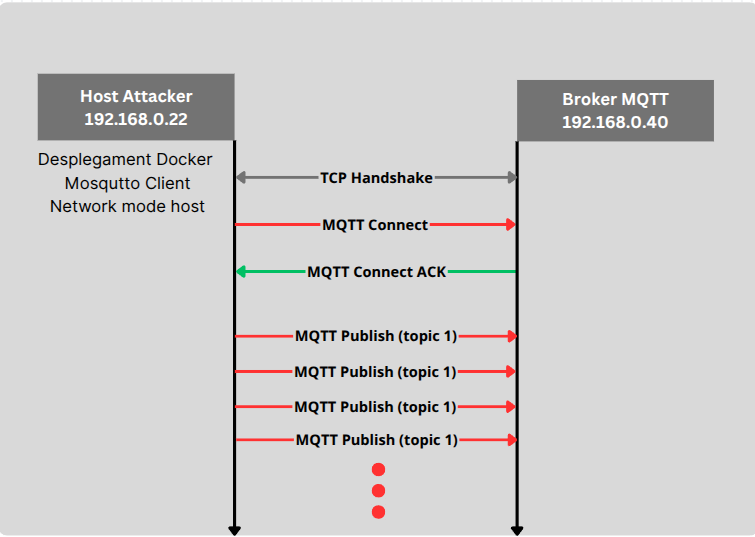
\includegraphics[width=1\textwidth]{img/DoSsimple.png}
    \caption{Esquema del trànsit generat per l'atac de denegació de servei MQTT Publish explicat anteriorment.}
    \label{fig:DoSsimple}
  \end{figure}


  \subsection{Denegació de servei Distribuïda (DDoS)}

Per a la realització d'atacs de denegació de servei en MQTT, és important entendre la persistència de les sessions en MQTT, explicada a \ref{sec:MQTT}. En l'atac DoS, si utilitzem sessions no persistents, cada vegada que l'atacant vol publicar un missatge, ha de tornar a intercanviar el handshake TCP i el handshake MQTT Connect. Els paquets intercanviats d'aquesta manera són lleugers i no generen una gran quantitat de trànsit, i, per tant, l'atac perd eficiència. En canvi, si s'utilitzen sessions persistents, els handshakes TCP i MQTT Connect només s'intercanvien una vegada i després es poden enviar missatges de forma contínua sense necessitat de tornar a establir la connexió.

L'atac proposat inicialment no és del tot realista, ja que la major part dels brokers MQTT, tenen configurats paràmetres per defecte per tal de limitar el nombre de missatges rebuts per segon des d'un client concret, com es pot veure a \ref{sec:mosquitto}. Per aquest motiu, vaig modificar l'script per tal que canviés el Client ID dels missatges en cada connexió.

El client ID és un identificador únic per a cada client MQTT que es connecta al broker. Si s'utilitza un Client ID diferent per a cada connexió, el broker no pot aplicar les mateixes restriccions de taxa de missatges, ja que cada connexió es veu com un client diferent. Aquest s'assigna a l'hora d'intercanviar els missatges MQTT Connect, per tant, no es pot fer l'atac amb connexions persistents, com he explicat anteriorment, es perd eficiència comparat amb l'atac anterior, això es pot veure comparant les quantitats de trànsit generades pels 2 atacs.

  \begin{figure}[H]
    \centering
    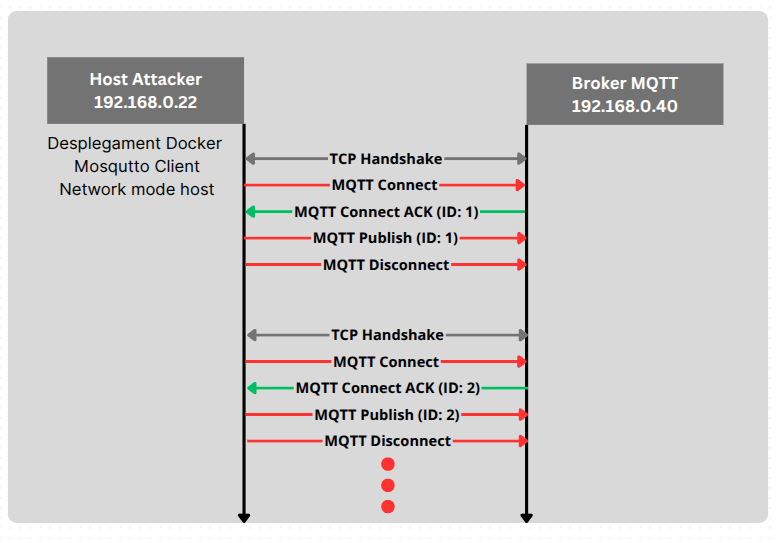
\includegraphics[width=1\textwidth]{img/DoSclientID.png}
    \caption{Esquema del trànsit generat per l'atac de denegació de servei MQTT Publish amb modificació del paràmetre Client ID.}
    \label{fig:DoSclientId}
  \end{figure}

El darrer mètode per a realitzar l'atac de denegació de servei distribuït amb Client ID diferents és mitjançant arquitectures de xarxa personalitzades amb Docker, concretament una arquitectura MACVLAN, on cada contenidor té una adreça IP diferent \ref{fig:DockerNetworks}. En aquesta versió de l'atac DDoS, generem un gran nombre de contenidors Docker i en cadascun despleguem un client MQTT. Aquests clients estableixen una connexió persistent amb el broker (amb Client ID diferents entre ells) i realitzen l'ataca de denegació de servei com els anteriors. Aquesta estratègia té una complexitat més elevada, però permet generar un gran nombre de connexions diferents però mantenint la persistència. D'aquesta manera, es s'aconsegueix un efecte similar a un DDoS amb diversos clients reals però utilitzant eines de virtualització com Docker.


  \begin{figure}[H]
    \centering
    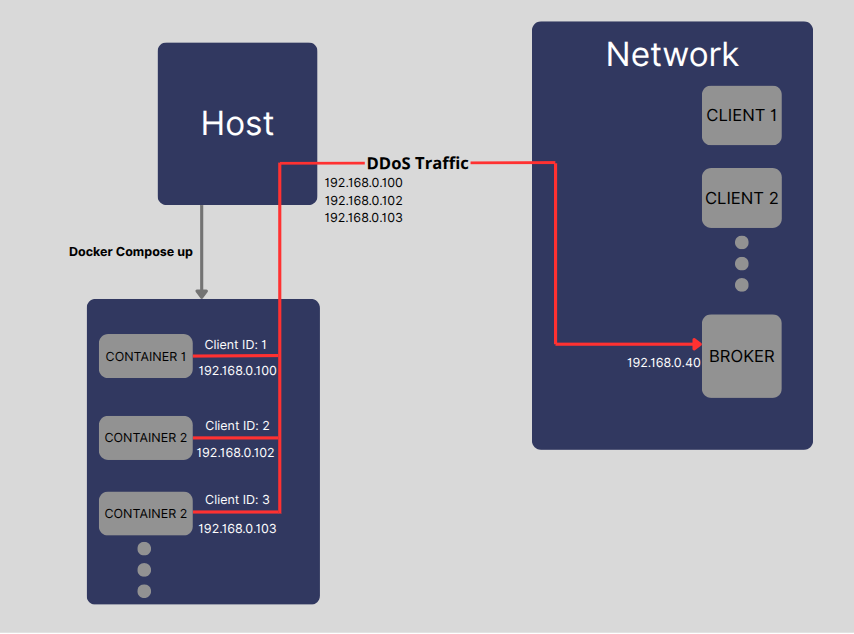
\includegraphics[width=1\textwidth]{img/DDoS.png}
    \caption{Esquema del trànsit generat per l'atac de denegació de servei Distribuït. El DDoS Traffic es refereix a trànsit generat amb una estructura similar al de la figura \ref{fig:DoSsimple}.}
    \label{fig:DDoS}
  \end{figure}

Un cop elaborat l'atac, he passat a utilitzar eines ja existents com ara "MQTTSA" i "MQTT Malaria" (\ref{sec:MQTTSA}) que ajuden a obtenir una eficiència més elevada al realitzar atacs DoS amb un codi més optimitzat. Aquestes tenen un funcionament similar al script de Python fet servir anteriorment.

També és molt important escollir el valor de QoS adequat per a l'atac, l'ús de QoS 0 permet enviar missatges sense esperar confirmació, per tant, permet saturar la xarxa amb mès facilitat, però, amb QoS 1, el processat que ha de realitzar el broker per a cada missatge és més elevat i, doncs, millora l'eficiència pel que fa a saturació del broker. Si s'utilitza QoS 2, aquest processat és encara més elevat i ja comporta una diferència molt notable respecte a QoS 0. Per tant, QoS 2 és l'opció més recomananada per a realitzar l'atac de denegació de servei. 

\subsection{Low-Rate DDoS}

Tal com s'explica a l'article \cite{lowrateDDoSexp}, els atacs de denegació de servei distribuïts (DDoS) poden ser realitzats amb un trànsit baix, és a dir, enviant un nombre reduït de missatges per segon. Aquest tipus d'atac pot ser més difícil de detectar i pot passar desapercebut per les mesures de seguretat del broker MQTT. Per a compensar la baixa taxa de missatges, s'utilitza un gran nombre de contenidors diferents, augmentant el nombre de clients.

  \begin{figure}[H]
    \centering
    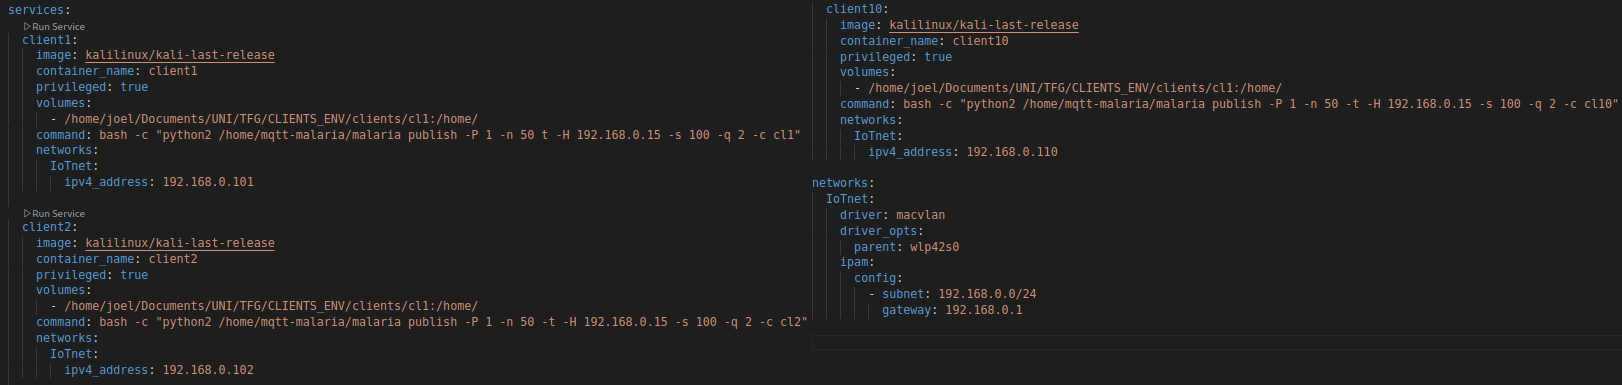
\includegraphics[width=1\textwidth]{img/lrDDoS.png}
    \caption{Arxiu yml utilitzat per Docker Compose per al desplegament de l'atac Low-Rate DDoS. S'utilitza un gran nombre de clients que executen peticions MQTT Publish mitjançant MQTT Malaria al broker amb IP 192.168.0.15 a un ritme realista.}
    \label{fig:LRDoS}
  \end{figure}